\documentclass[12pt, a4paper]{article}
\usepackage[bottom=2cm,top=3cm,left=3cm,right=2cm]{geometry}
\usepackage[brazilian]{babel} % Traduz alguns termos para o português
\usepackage[utf8]{inputenc} % Reconhece acentuação
\usepackage{color,graphicx}
\usepackage{enumerate}
\usepackage{mathtools}
\usepackage{listings}
\usepackage{longtable}
\usepackage[section]{placeins}
\usepackage[hidelinks=true]{hyperref}
\hypersetup{
	colorlinks=false,     
	urlcolor=blue
}

\definecolor{olive}{RGB}{175,128,0}
\definecolor{Aquamarine}{RGB}{0,175,175}

\usepackage{setspace}
\onehalfspacing	
\setlength{\parindent}{30pt}

\usepackage{indentfirst}

\title{
	\begin{large}
		Estudo de Caso 03: Emparelhamento de dados
	\end{large}	}
\author{Gustavo Vieira Costa - 2010022003\\Marcus Vinícius - 2013030147\\Rafael Castro - 2013030210\\Thaís Matos Acácio - 2013030287}
\date{25/04/2016}

\begin{document}
	\maketitle
	
	\vspace*{-8.5cm}
	{\bf
		\begin{center}
			{\large
				\hspace*{0cm}Universidade Federal de Minas Gerais} \\
			\hspace*{0cm}Engenharia de Sistemas  \\
		\end{center}
	}
	\vspace*{5cm}
	
\section{Introdução}
Uma percepção comum é a de que pessoas tendem a sistematicamente declarar um peso corporal inferior ao valor real. Com base nessa afirmação, iremos investigar o viés de relato de peso dos alunos de Engenharia de Sistemas, mediante comparação dos valores estimados pelos alunos da disciplina com valores aferidos por uma balança digital de uso doméstico.
\par O experimento realizado utiliza o conceito de emparelhamento de dados, no qual a hipótese a ser testada passa a ser relacionada com a diferença entre as médias da amostra.

\section{Coleta de dados}
A Tabela \ref{table:amostra} contém a amostra de dados coletada, ou seja, o peso informados pelos alunos da disciplina e aferidos pela balança, juntamente com um identificador aleatório e único para cada um dos alunos:
\par Os valores dos pesos declarados e medidos foram exibidos no gráfico de blocos \ref{fig:blocos} para possibilitar uma melhor visualização do comportamento da amostra. O diagrama \ref{fig:blocos_diff} retrata a diferença entre esses valores.
\pagebreak
\begin{longtable}{|c|c|c|c|c|}
\hline
\rule[-1.0ex]{0pt}{4.0ex}
\textbf{ID}&\textbf{Peso Estimado(kg)}&\textbf{Peso Medido(kg)}\\ \hline
\endhead
\rule[-1.0ex]{0pt}{4.0ex}
EngSis.A&78.4&79.6 \\ \hline
\rule[-1.0ex]{0pt}{4.0ex}
EngSis.B&69.5&69.3 \\ \hline
\rule[-1.0ex]{0pt}{4.0ex}
EngSis.C&66.2&66.4 \\ \hline
\rule[-1.0ex]{0pt}{4.0ex}
EngSis.D&61.0&60.4 \\ \hline
\rule[-1.0ex]{0pt}{4.0ex}
EngSis.E&59.0&57.7 \\ \hline
\rule[-1.0ex]{0pt}{4.0ex}
EngSis.F&70.5&71.3 \\ \hline
\rule[-1.0ex]{0pt}{4.0ex}
EngSis.G&63.5&63.3 \\ \hline
\rule[-1.0ex]{0pt}{4.0ex}
EngSis.H&81.0&79.3 \\ \hline
\rule[-1.0ex]{0pt}{4.0ex}
EngSis.I&57.7&53.5 \\ \hline
\rule[-1.0ex]{0pt}{4.0ex}
EngSis.J&49.0&52.0 \\ \hline
\rule[-1.0ex]{0pt}{4.0ex}
EngSis.K&68&71.7 \\ \hline
\caption{Tabela de Amostras}
\label{table:amostra}
\end{longtable}
\begin{figure}[h]
\centering
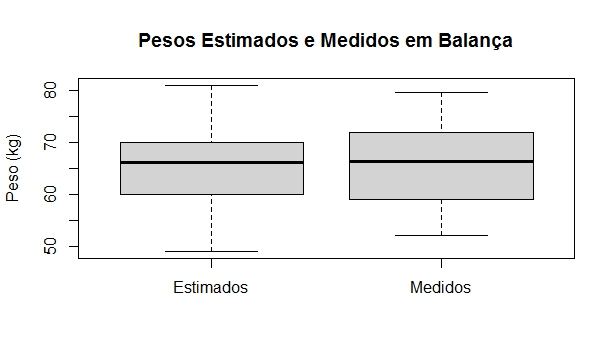
\includegraphics[scale=0.6]{img/box.jpeg}
\caption{Pesos Estimados e Medidos}
\label{fig:blocos}
\end{figure}
\begin{figure}[h]
\centering
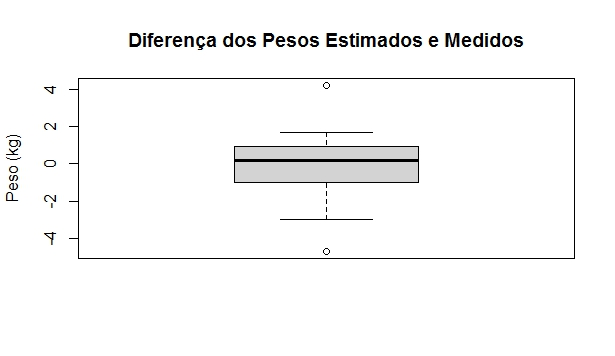
\includegraphics[scale=0.6]{img/box_diff.jpeg}
\caption{Diferença dos Pesos Estimados e Medidos}
\label{fig:blocos_diff}
\end{figure}
\par De acordo com o \textit{Teorema do Limite Central}, se a amostra tiver tamanho n suficiente, a distribuição amostral de $\bar{x}$ é aproximadamente Normal. Nesse caso, iremos assumir que n é suficiente, conforme o gráfico de normalidade presente na figura \ref{fig:normal}.
%\begin{figure}[h]
%\centering
%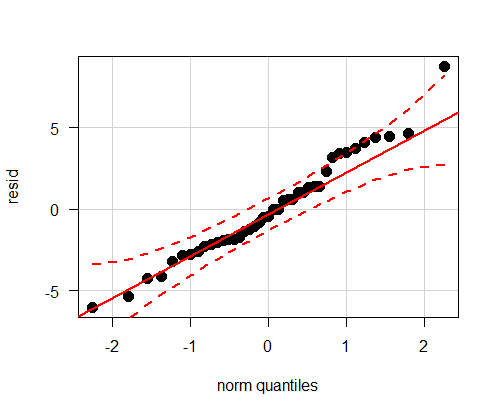
\includegraphics[scale=0.8]{img/plot-normalidade.png}
%\caption{Normalidade das amostras}
%\label{fig:normal}
%\end{figure}

\section{Estratégia de Inferência}
\label{sec:estrategia-inferencia}
O processo de inferência estatística consiste em tirar conclusões sobre uma população com base em informações extraídas de amostras da mesma. No presente estudo de caso, o parâmetro sobre o qual temos interesse é a média das diferenças entre os pesos medidos e estimados $\mu_{D}$ dos alunos de graduação em Engenharia de Sistemas.
\par O método se baseia em calcular a diferença entre cada par de pesos estimado e medido de cada aluno, determinar a média dessas diferenças e informar se essa média é estatisticamente significativa. Podemos utilizar o método de inferência para uma única amostra, visto que temos apenas duas observações de uma mesma amostra, as quais serão pareadas.
\newline
\newline
\textbf{Premissas do Teste}
\begin{itemize}
\item O \textbf{nível de significância}($\alpha$), representa a probabilidade de erro tipo I, ou seja, a probabilidade de rejeitarmos a hipótese nula quando ela é efetivamente verdadeira. Pensando em uma taxa de erro aceitável para o domínio do problema, fixamos $\alpha = 0.05$.
\item $\beta$ representa a \textbf{probabilidade de erro tipo II}, ou seja, aceitarmos a hipótese nula quando ela é efetivamente falsa. Resolvemos permitir um erro tipo II de $20\%$ ($\beta = 0.2$), considerando que esse tipo de erro tem menor impacto negativo do que o erro tipo I.
\item \textbf{Nível de confiança} ($1 - \alpha$) tem como objetivo conhecer o quanto o teste de hipóteses controla um erro do tipo I, ou qual a probabilidade de aceitar a hipótese nula se realmente for verdadeira. 
\item O \textbf{poder do teste} ($1 - \beta$) tem como objetivo conhecer o quanto o teste de hipóteses controla um erro do tipo II ou, qual a probabilidade de rejeitar a hipótese nula se realmente for falsa.
\item O menor \textbf{tamanho de efeito} de importância prática($\delta^*$) como 0.5, considerando o peso médio das roupas e umerro de precisão aceitável para a balança.
\end{itemize}

\textbf{Hipóteses de Teste}
\par O teste estatístico é planejado para avaliar a força da evidência \textit{contra} a hipótese nula $H_{0}$. Usualmente, a hipótese nula é uma afirmativa de "nenhum efeito". A afirmativa sobre a população \textit{a favor} da qual estamos tentando achar evidência é a hipótese alternativa $H_{1}$. Logo, as hipóteses são:
\begin{equation}
\left \{
\begin{array}{cc}
H_{0}: & \mu_{D} = 0 \\
H_{1}: & \mu_{D} \neq 0 \\
\end{array}
\right.
\end{equation}
\newline sendo $\mu_{D}$ a média das diferenças, entre os pesos estimados e medidos, dos alunos de Engenharia de Sistemas.

\section{Projeto experimental e Análise dos Resultados}
\label{sec:projeto-experimental}

\section{Conclusão}

\begin{thebibliography}{6}
\bibitem{1}{\url{https://github.com/fcampelo/Design-and-Analysis-of-Experiments}}
\bibitem{2}{Estatística Aplicada e Probabilidade para Engenheiros (4ª edição) - Montgomery}
\bibitem{3}{A Estatística Básica e Sua Prática (6ª edição) - David S. Moore, William I. Nortz, Michael A. Fligner}
\bibitem{4}{\url{https://stat.ethz.ch/R-manual/R-devel/library/stats/html/var.test.html}}
\bibitem{5}{\url{http://ww2.coastal.edu/kingw/statistics/R-tutorials/independent-t.html}}
\bibitem{6}{\url{http://www.portalaction.com.br/inferencia/56-teste-para-comparacao-de-duas-variancias-teste-f}}
\end{thebibliography}		
		
\end{document}